\documentclass[a4paper]{article}
\usepackage[left=3cm,right=3cm,top=2cm,bottom=2cm]{geometry} % page settings
\usepackage{enumerate}
\usepackage{hyperref}
\usepackage{graphicx}
\usepackage{amsfonts}
\usepackage{amsthm}
\usepackage{mathtools}
\usepackage{titlesec}
\usepackage{polski}
\usepackage{tikz}
\usepackage[utf8]{inputenc}
\DeclarePairedDelimiter\ceil{\lceil}{\rceil}
\DeclarePairedDelimiter\floor{\lfloor}{\rfloor}
\DeclarePairedDelimiter\set{\lbrace}{\rbrace}


\def\checkmark{\tikz\fill[scale=0.3](0,.35) -- (.25,0) -- (1,.7) -- (.25,.15) -- cycle;} 

\titlespacing*{\subsection}
{0ex}{10ex}{3ex}

\title{Lista 1}
\author{Kamil Matuszewski}
\date{13 marca 2016}

\begin{document}

\maketitle
\setlength{\parindent}{0.5ex}
\setlength{\parskip}{1.5ex}
\newcommand{\R}{\mathbb{R}}
\newcommand{\N}{\mathbb{N}}


\begin{center}
\begin{tabular}{|c *{8}{|c} |c|}\hline
1 & 2 & 3 & 4 & 5 & 6 & 7 & 8 & 9\\
\hline 
\checkmark &\checkmark &\checkmark &\checkmark &\checkmark &\checkmark &\checkmark &\checkmark &\\
\hline
\end{tabular}
\end{center}


\subsection*{Zadanie 1}
Dla każdego z podanych poniżej adresów IP w notacji CIDR określ, czy jest to adres sieci, adres rozgłoszeniowy czy też adres komputera. W każdym przypadku wyznacz odpowiadający mu adres sieci,rozgłoszeniowy i jakiś adres IP innego komputera w tej samej sieci.

\begin{itemize}
\item 10.1.2.3/8 - Adres sieci: 10.0.0.0, adres rozgłoszeniowy: 10.255.255.255, \textbf{jakiś adres:}10.1.2.4
\item 156.17.0.0/16 - \textbf{Adres sieci}:156.17.0.0 adres rozgłoszeniowy:156.17.255.255, jakiś adres: 156.17.69.0
\item 99.99.99.99/27 - Adres sieci:99.99.99.96, adres rozgłoszeniowy: 99.99.99.127, \textbf{jakiś adres} 99.99.99.111
\item 156.17.64.4/30 - \textbf{Adres sieci}: 156.17.64.4, adres rozgłoszeniowy 156.17.64.7, jakiś adres: 156.17.64.6
\item 123.123.123.123 - \textbf{Sieć z jednym ip, to jedno jest wszystkim}
\end{itemize}

\subsection*{Zadanie 2}
Podziel sieć 10.10.0.0/16 na 5 rozłącznych podsieci, tak żeby każdy z adresów IP z sieci 10.10.0.0/16 był
w jednej z tych 5 podsieci. Jak zmieniła się liczba adresów IP możliwych do użycia przy adresowaniu
komputerów? Jaki jest minimalny rozmiar podsieci, który możesz uzyskać w ten sposób?


Adres sieci: 00001010.00001010.00000000.00000000, maska: 11111111.11111111.00000000.00000000. Dzielimy sieć na podsieci:\\
\begin{itemize}
\item Adres sieci: 00001010.00001010.00000000.00000000, maska: 11111111.11111111.10000000.00000000 tzn 10.10.0.0/17
\item Adres sieci: 00001010.00001010.10000000.00000000, maska: 11111111.11111111.11000000.00000000 tzn 10.10.128.0/18
\item Adres sieci: 00001010.00001010.11000000.00000000, maska: 11111111.11111111.11100000.00000000 tzn 10.10.192.0/19
\item Adres sieci: 00001010.00001010.11100000.00000000, maska: 11111111.11111111.11110000.00000000 tzn 10.10.224.0/20
\item Adres sieci: 00001010.00001010.11110000.00000000, maska: 11111111.11111111.11110000.00000000 tzn 10.10.240.0/20


\end{itemize}
Czyli podzieliliśmy sieć na pół, z jednej połowy zrobiliśmy pierwszą podsieć, drugą podzieliliśmy na pół, i z pierwszej połowy zrobiliśmy drugą podsieć, drugą podzieliliśmy na pół itd.

Każdy adres potrzebuje adresu podsieci i adresu rozgłoszeniowego. Mamy 5 podsieci, stąd 10 adresów nam "przepada" i nie możemy ich użyć do adresowania komputerów. Ale nasza oryginalna sieć miała już jakiś adres rozgłoszeniowy i adres sieci które możemy wykorzystać na nasze podsieci, stąd w rzeczywistości straciliśmy 8 adresów ip.

Minimalny adres podsieci na jaką mogę podzielić sieć to 1: przydzieliłbym dokładnie jeden adres ip dla tej podsieci.

\subsection*{Zadanie 3}
Tablica routingu zawiera następujące wpisy (podsieć $\rightarrow$ dokąd wysłać):
\begin{itemize}
\item 0.0.0.0/0 $\rightarrow$ do routera A
\item 10.0.0.0/23 $\rightarrow$ do routera B
\item 10.0.2.0/24 $\rightarrow$ do routera B
\item 10.0.3.0/24 $\rightarrow$ do routera B
\item 10.0.1.0/24 $\rightarrow$ do routera C
\item 10.0.0.128/25 $\rightarrow$ do routera B
\item 10.0.1.8/29 $\rightarrow$ do routera B
\item 10.0.1.16/29 $\rightarrow$ do routera B
\item 10.0.1.24/29 $\rightarrow$ do routera B
\end{itemize}
Napisz równoważną tablicę routingu zawierającą jak najmniej wpisów

Wiemy, że w tablicy routingu jeśli pasuje więcej niż jedna reguła, wybierana jest ta najkonkretniejsza. Wykorzystajmy to.

\begin{itemize}
\item 0.0.0.0/0 $\rightarrow$ do routera A
\item 10.0.0.0/22 $\rightarrow$ do routera B
\item 10.0.1.0/24 $\rightarrow$ do routera C
\item 10.0.1.0/27 $\rightarrow$ do routera B
\item 10.0.1.0/29 $\rightarrow$ do routera C
\end{itemize}

\clearpage
\subsection*{Zadanie 4}
Wykonać powyższe zadanie dla tablicy

\begin{itemize}
\item 0.0.0.0/0 $\rightarrow$ do routera A
\item 10.0.0.0/8 $\rightarrow$ do routera B
\item 10.3.0.0/24 $\rightarrow$ do routera C
\item 10.3.0.32/27 $\rightarrow$ do routera B
\item 10.3.0.64/27 $\rightarrow$ do routera B
\item 10.3.0.96/27 $\rightarrow$ do routera B
\end{itemize}

To samo co wyżej

\begin{itemize}
\item 0.0.0.0/0 $\rightarrow$ do routera A
\item 10.0.0.0/8 $\rightarrow$ do routera B
\item 10.3.0.0/24 $\rightarrow$ do routera C
\item 10.3.0.0/25 $\rightarrow$ do routera B
\item 10.3.0.0/27 $\rightarrow$ do routera C
\end{itemize}

\clearpage
\subsection*{Zadanie 5}
Krok 0\\
\begin{tabular}{|c *{6}{|c} |c|}\hline
 & A & B & C & D & E & F\\
\hline 
do A & - & 1 & & & &\\
\hline 
do B & 1 & - & 1 & & &\\
\hline 
do C & & 1 & - & & 1 & 1\\
\hline 
do D & & & & - & 1 &\\
\hline 
do E & & & 1 & 1 & - & 1\\
\hline
do F & & & 1 & & 1 & -\\
\hline
\end{tabular}

Krok 1\\
\begin{tabular}{|c *{6}{|c} |c|}\hline
 	 & A & B & C 		 & D & E & F\\
\hline 
do A & - & 1 & 2 (Via B) & & &\\
\hline 
do B & 1 & - & 1 		 & & 2 (Via C) & 2 (Via C)\\
\hline 
do C & 2 (Via B) & 1 & - & 2 (Via E) & 1 & 1\\
\hline 
do D & & & 2 (Via E) & - & 1 & 2 (Via E)\\
\hline 
do E & & 2 (Via C) & 1 & 1 & - & 1\\
\hline
do F & & 2 (Via C) & 1 & 2 (Via E) & 1 & -\\
\hline
\end{tabular}

Krok 2\\
\begin{tabular}{|c *{6}{|c} |c|}\hline
 & A & B & C & D & E & F\\
\hline 
do A & - & 1 & 2 (Via B) &  & 3 (Via C) &  3 (Via C)\\
\hline 
do B & 1 & - & 1 & 3 (Via E) & 2 (Via C) & 2 (Via C)\\
\hline 
do C & 2 (Via B) & 1 & - & 2 (Via E) & 1 & 1\\
\hline 
do D & 			 & 3 (Via C) & 2 (Via E) & - & 1 & 2 (Via E)\\
\hline 
do E & 3 (Via B) & 2 (Via C) & 1 & 1 & - & 1\\
\hline
do F & 3 (Via B) & 2 (Via C) & 1 & 2 (Via E) & 1 & -\\
\hline
\end{tabular}

Krok 3\\
\begin{tabular}{|c *{6}{|c} |c|}\hline
 & A & B & C & D & E & F\\
\hline 
do A & - & 1 & 2 (Via B) & 4 (Via E)  & 3 (Via C) &  3 (Via C)\\
\hline 
do B & 1 & - & 1 & 3 (Via E) & 2 (Via C) & 2 (Via C)\\
\hline 
do C & 2 (Via B) & 1 & - & 2 (Via E) & 1 & 1\\
\hline 
do D & 4 (Via B) & 3 (Via C) & 2 (Via E) & - & 1 & 2 (Via E)\\
\hline 
do E & 3 (Via B) & 2 (Via C) & 1 & 1 & - & 1\\
\hline
do F & 3 (Via B) & 2 (Via C) & 1 & 2 (Via E) & 1 & -\\
\hline
\end{tabular}

\clearpage
\subsection*{Zadanie 6}
Załóżmy, że dodamy połączenie między A i D. Jak zmieni się sytuacja?

Krok 0\\
\begin{tabular}{|c *{6}{|c} |c|}\hline
 & A & B & C & D & E & F\\
\hline 
do A & - & 1 & 2 (Via B) & 1  & 3 (Via C) &  3 (Via C)\\
\hline 
do B & 1 & - & 1 & 3 (Via E) & 2 (Via C) & 2 (Via C)\\
\hline 
do C & 2 (Via B) & 1 & - & 2 (Via E) & 1 & 1\\
\hline 
do D & 1 & 3 (Via C) & 2 (Via E) & - & 1 & 2 (Via E)\\
\hline 
do E & 3 (Via B) & 2 (Via C) & 1 & 1 & - & 1\\
\hline
do F & 3 (Via B) & 2 (Via C) & 1 & 2 (Via E) & 1 & -\\
\hline
\end{tabular}

Krok 1\\
\begin{tabular}{|c *{6}{|c} |c|}\hline
 & A & B & C & D & E & F\\
\hline 
do A & - & 1 & 2 (Via B) & 1 & 2 (Via D) &  3 (Via C)\\
\hline 
do B & 1 & - & 1 & 2 (Via A) & 2 (Via C) & 2 (Via C)\\
\hline 
do C & 2 (Via B) & 1 & - & 2 (Via E) & 1 & 1\\
\hline 
do D & 1 & 2 (Via A) & 2 (Via E) & - & 1 & 2 (Via E)\\
\hline 
do E & 2 (Via D) & 2 (Via C) & 1 & 1 & - & 1\\
\hline
do F & 3 (Via B) & 2 (Via C) & 1 & 2 (Via E) & 1 & -\\
\hline
\end{tabular}

\subsection*{Zadanie 7}
Troszku opisowo:

Wszystko działa spoko, ale nagle psuje się łącze między C i E. W takim razie C wysyła komunikat do B i D: \textbf{mam do E ścieżkę nieskończoną}.\\
B i D reagują na to zmianą ścieżki do E. Wysyłają do A wiadomość: \textbf{mam do E ścieżkę nieskończoną + 1}. A aktualizuje swoje informacje. Wszystko działa.

Jednak, co jeśli to A wyśle pierwsze komunikat do B i D? Powie im: \textbf{mam do E ścieżkę długości 3}. Wtedy B i D pomyślą: tak jest szybciej, więc idziemy tamtędy. Aktualizują swoją informację i rozsyłają dookoła: \textbf{mam do E ścieżkę długości 4}. W kolejnym kroku zauważa to C. Pojawiła się krótsza ścieżka do E. Mówi więc: \textbf{mam do E ścieżkę długości 5}. Jednak w tym samym kroku A zauważa, że coś się popsuło: wcześniejsze połączenie przez B/D zwiększyło się o 1. Wysyła więc informacje: \textbf{mam do E ścieżkę długości 4}. W kolejnym kroku B i D dowiadują się, że ścieżka do E zwiększyła się o 1. Zwiększają więc swoją ścieżkę o 1 i rozsyłają informację dookoła... W kolejnym kroku ścieżkę zwiększą A i C, w kolejnym B i D... I tak w kółko. Mamy cykl.
\clearpage
\subsection*{Zadanie 8}
Pokaż, że przy wykorzystaniu algorytmu stanu łączy też może powstać cykl w routingu.

Spójrzmy na rysunek:\\
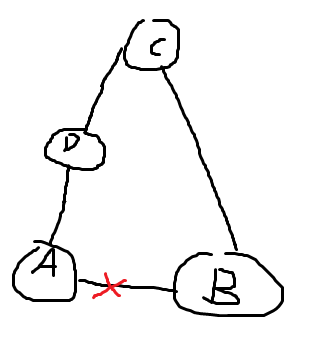
\includegraphics[scale=0.7]{zad8.png}

Ok. Więc C wie, że najszybsza droga pakietów do A może przekazywać przez B. Nagle łącze A-B się psuje. B chce wysłać pakiet do A - musi to zrobić przez C. Wysyła więc pakiet do A przez C, aktualizując u siebie informację, że nie ma już sąsiada A. Informacja ta się rozchodzi - jednak może się rozchodzić wolniej, niż idzie pakiet (sporo trzeba zaktualizować w każdym ruterze, obliczyć jeszcze raz najkrótsze ścieżki itd). Może się zdarzyć, że C otrzyma pakiet, i zauważa, że najszybciej dostarczy go przez B - więc wysyła go do B. B jednak musi go przesłać przez C, bo to jedyna droga. Mamy cykl. Nie wiem czy o to chodziło bo to w końcu nie jest cykl nieskończony... Ale nim informacja o braku połączenia między A i B dotrze do C pakiet będzie biegać w tą i z powrotem, a z treści wynika, że o to chodziło (Pokaż, że w okresie
propagowania tej aktualizacji (kiedy dotarła ona już do części routerów a do części nie) może powstać
cykl w routingu).

\end{document}
